\section{Anwendungen}
\subsection{Digitalisierung}
\subsection{Auflösung}
Die A/D Auflösung in bit $n$ eines Sensor kann durch folgende Formel berechnet werden, falls Aufteilung linear ist:
\[
n = \lceil \log_2\left(\frac{\Delta}{a}\right) \rceil
\]
\textbf{Beispiel:}
$a = 1.0g$ und Messung von $0kg...20kg$ ergibt $15bit = \lceil \log_2\left(\frac{20000g}{1g}\right) \rceil$

\begin{center}
	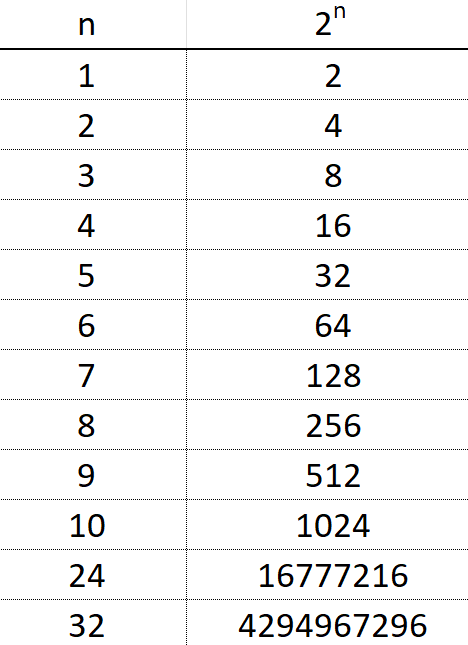
\includegraphics[width=0.4\columnwidth]{Images/zweierpotenz}
\end{center}
\noindent Beispiel für $20'000 \leq 2^{10}\cdot2^5 \xrightarrow{} 10 + 5bit$

\subsection{DGL von Model}
Am besten wird bei der höchsten Ableitung in einem Diagram beginnen. Allenfalls Hilfsvariablen erstellen.

\noindent\textbf{Beispiel 1:}
\begin{center}
	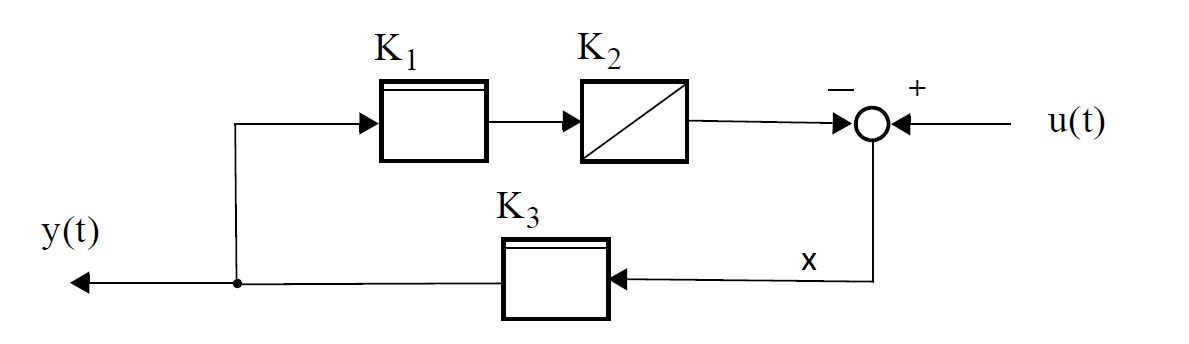
\includegraphics[width=0.8\columnwidth]{Images/dgl_bestimmen}
\end{center}
\begin{align*}
	x &= u - K_1K_2\int y dt \qquad y = K_3x \\
	y &= K_3\left[u - K_1K_2\int y dt\right] \\
	y &= K_3u - K_1K_2K_3\int y dt \\ 
	\dot{y} + K_1K_2K_3 y &= K_3 \dot{u}
\end{align*}

\noindent\textbf{Beispiel 2:}
\begin{center}
	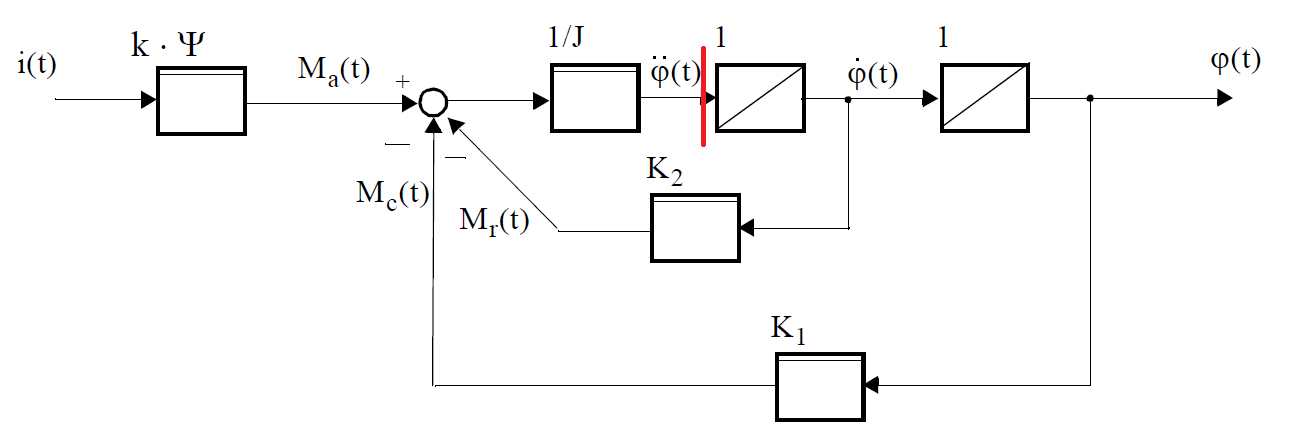
\includegraphics[width=0.8\columnwidth]{Images/dgl_bestimmen1}
\end{center}
\begin{align*}
	\ddot{\varphi} = \left(-K_2\dot\varphi - K_1\varphi + k\Psi i\right)\frac{1}{J}\\
	J\ddot{\varphi} + K_2\dot\varphi + K_1\varphi = k \Psi i
\end{align*}

\subsection{Zahnrad}
Dabei kann der Übersetzungsfaktor $n = \frac{Z2}{Z1}$ berechnet werden und Offset $O$ von entsprechendem Winkel hinzu addiert werden.
\begin{center}
	\begin{minipage}{0.35\textwidth}
		\begin{center}
			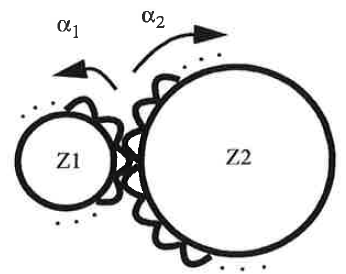
\includegraphics[width=0.25\linewidth,keepaspectratio=true]{Images/zahnrad_I}
			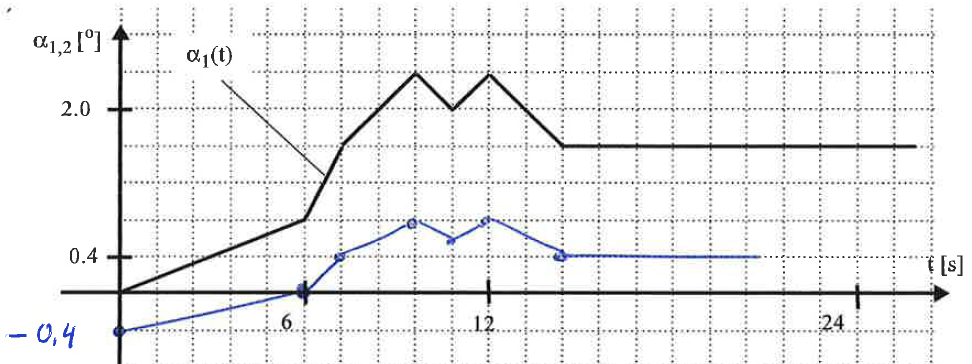
\includegraphics[width=0.5\linewidth,keepaspectratio=true]{Images/zahnrad_I1}
		\end{center}
	\end{minipage}%%% to prevent a space
	\begin{minipage}{0.15\textwidth}
		\begin{align*}
			\alpha_2 = \frac{\Delta \alpha_1}{n} + O
		\end{align*}
	\end{minipage}
\end{center}

\begin{center}
	\begin{minipage}{0.35\textwidth}
		\begin{center}
			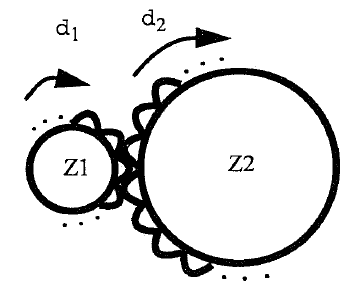
\includegraphics[width=0.25\linewidth,keepaspectratio=true]{Images/zahnrad_II}
			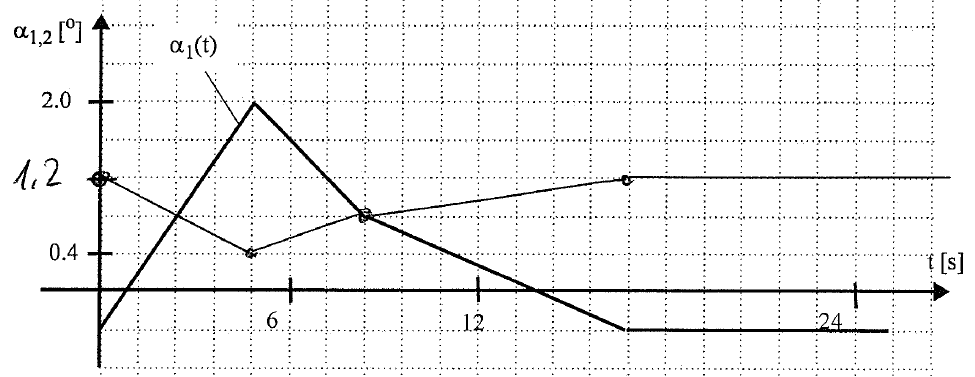
\includegraphics[width=0.5\linewidth,keepaspectratio=true]{Images/zahnrad_II2}
		\end{center}
	\end{minipage}%%% to prevent a space
	\begin{minipage}{0.15\textwidth}
		\begin{align*}
			\alpha_2 = -\frac{\Delta\alpha_1}{n} + O
		\end{align*}
	\end{minipage}
\end{center}

\subsection{Arbeitspunkt}
Um ein \textbf{Arbeitspunkt} bzw die \textbf{statische Analyse} zu erhalten werden die höheren Ableitungen Null gesetzt und die Gleichung gelöst.\\~\\
\noindent Mit folgendem Schema und Nominalwerte $u=u_0=2$ und $z=z_0 = 3$\\
\begin{center}
	\begin{minipage}{0.20\textwidth}
		\begin{center}
			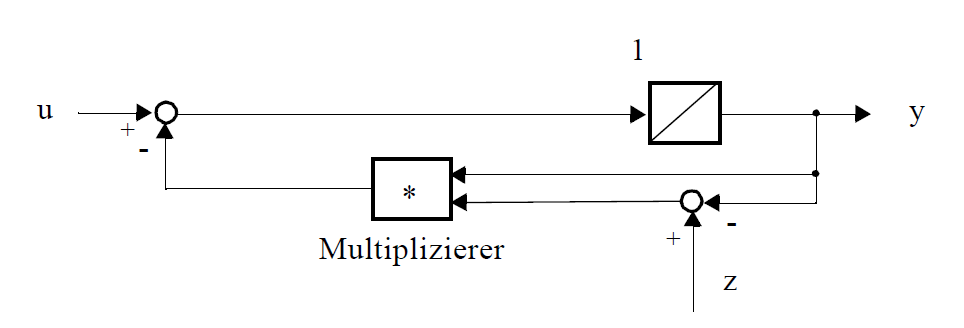
\includegraphics[width=\linewidth,keepaspectratio=true]{Images/arbeitspunkt}\\
		\end{center}
	\end{minipage}%%% to prevent a space
	\begin{minipage}{0.3\textwidth}
\begin{align*}
	&\dot{y} &= u - y(-y + z) \qquad (\dot{y} &\eqi 0) \\ \\
	\Rightarrow& & u - y(-y + z) &= 0\\
	&&y^2 - 3y +2 &= 0 \\
\end{align*}
Die Arbeitspunkte sind $\mathbb{L} = \{1, 2\}$
	\end{minipage}
\end{center}

\subsection{Exp-Funktion} 
\begin{center}
	$e^{-\frac{t}{a}}$\\
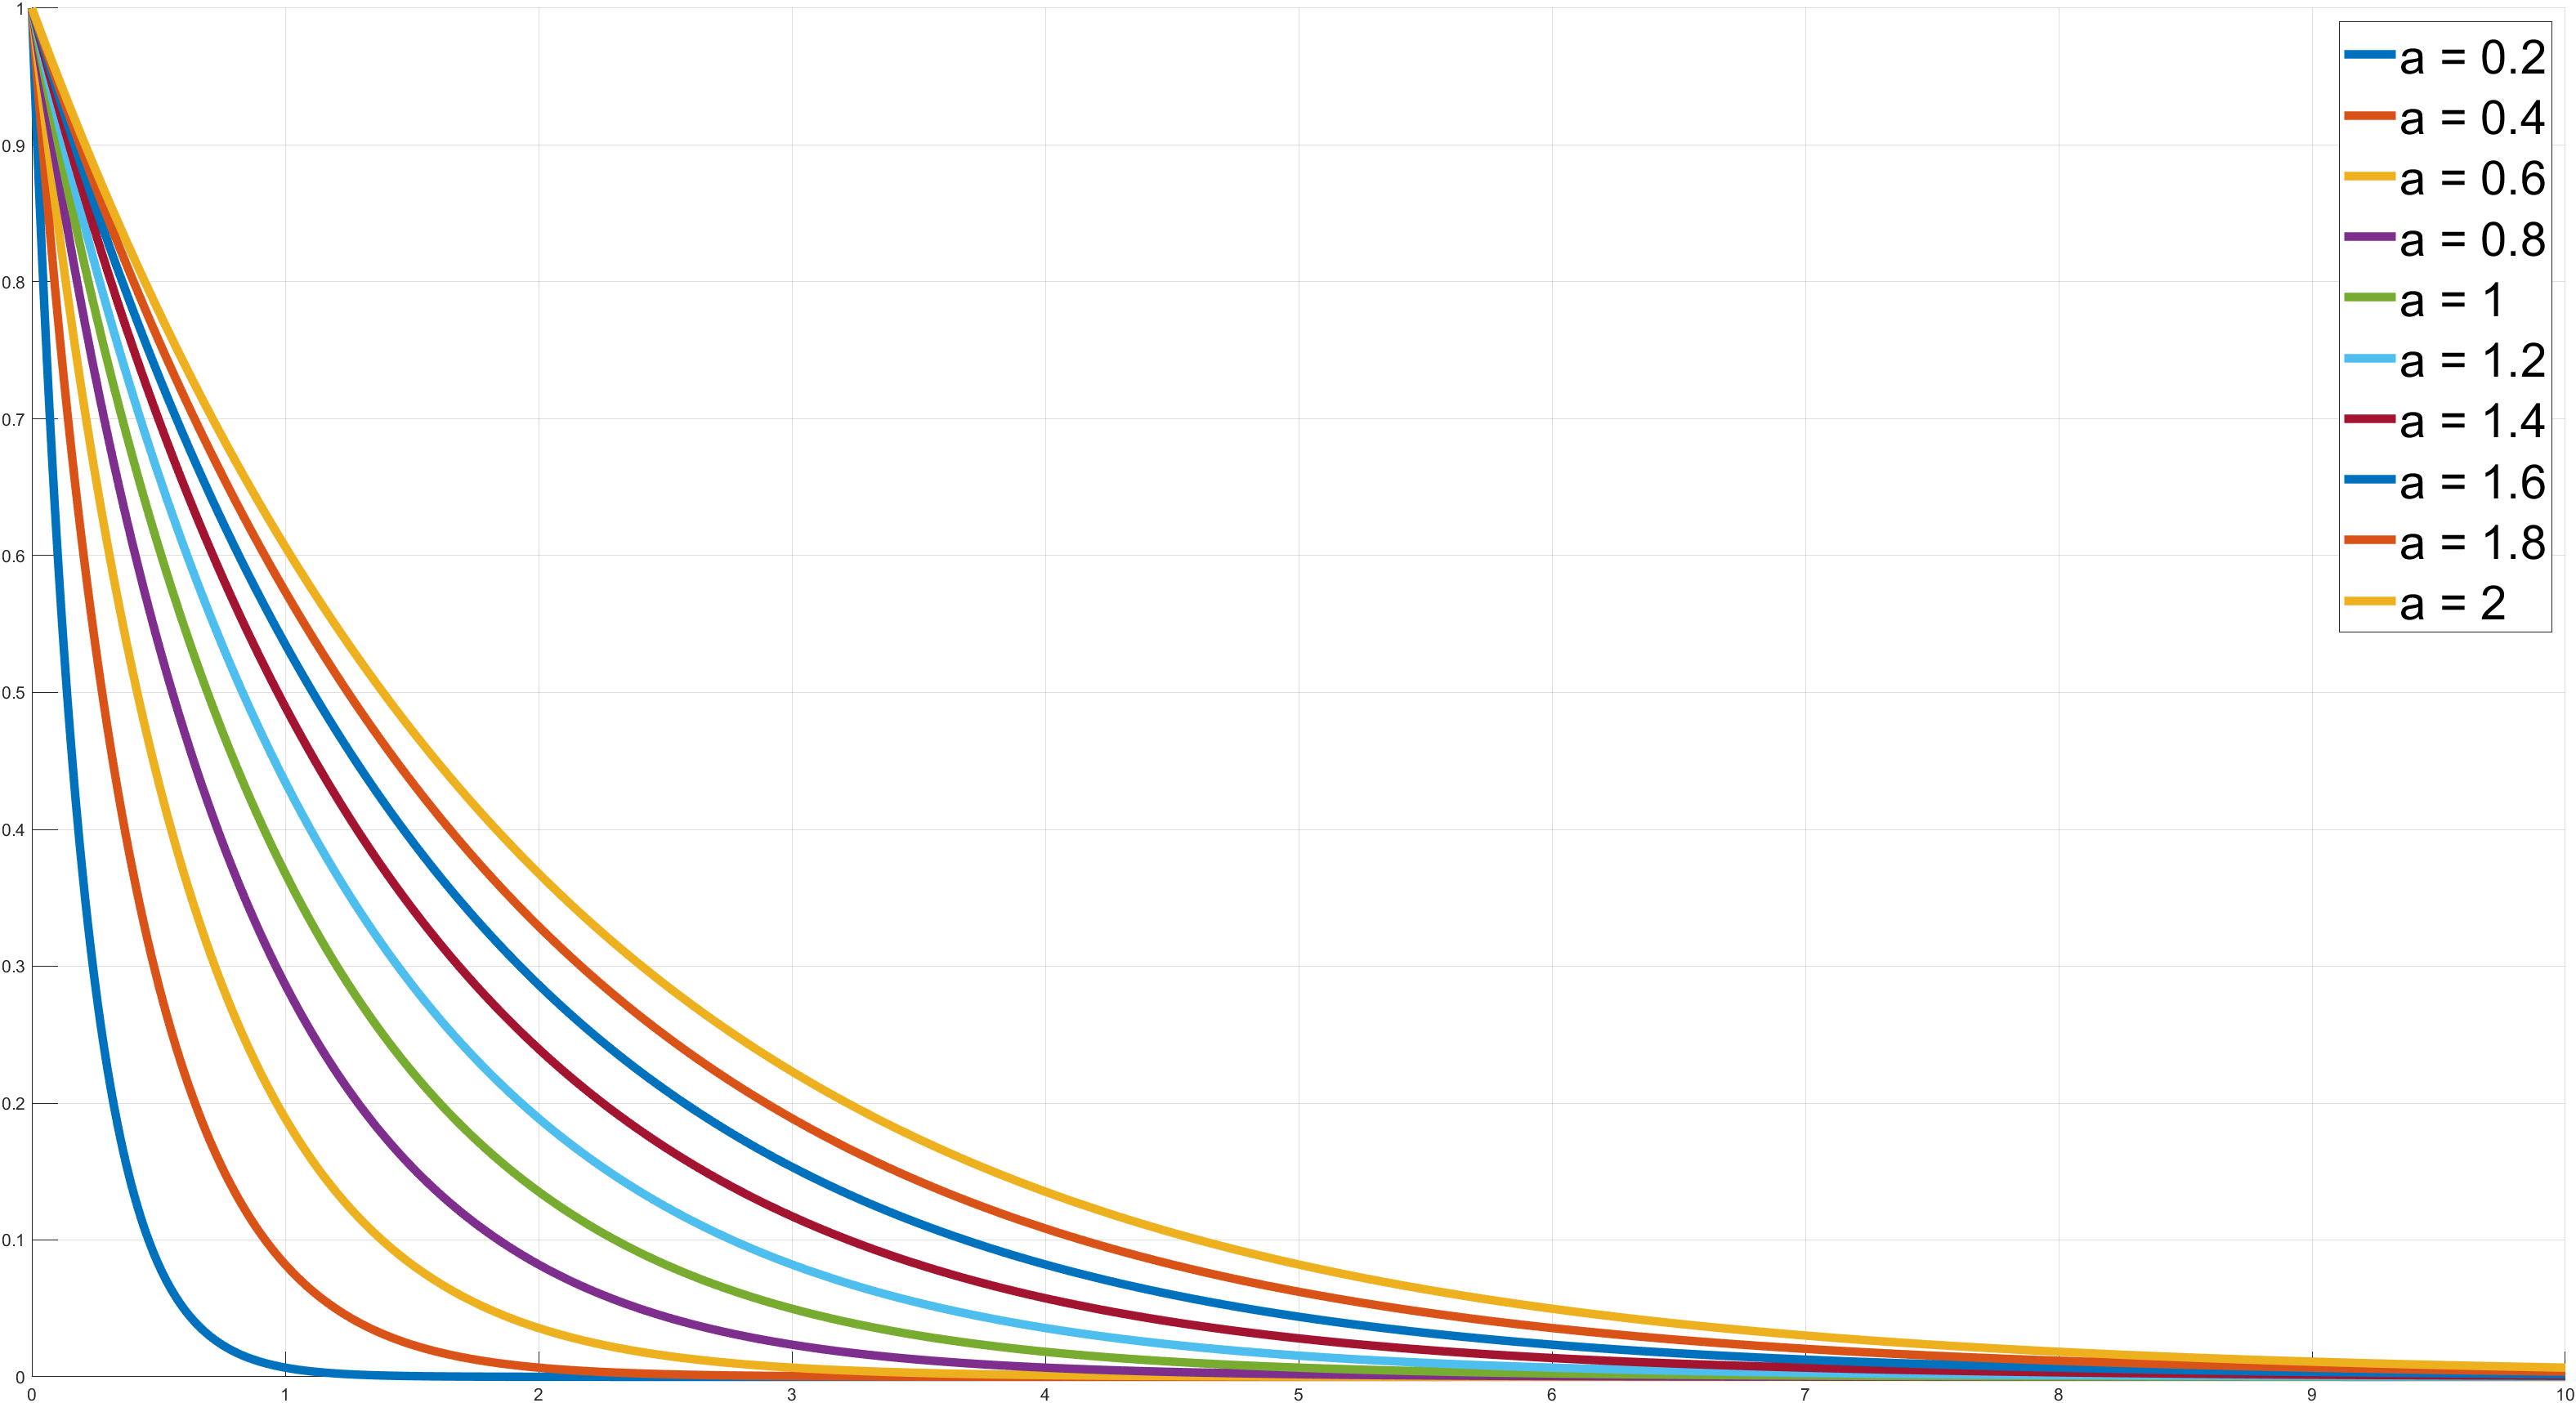
\includegraphics[width=\linewidth,keepaspectratio=true]{Images/exp}
\end{center}



